\documentclass{standalone}
\usepackage{tikz}
\usetikzlibrary{patterns, positioning}


\begin{document}
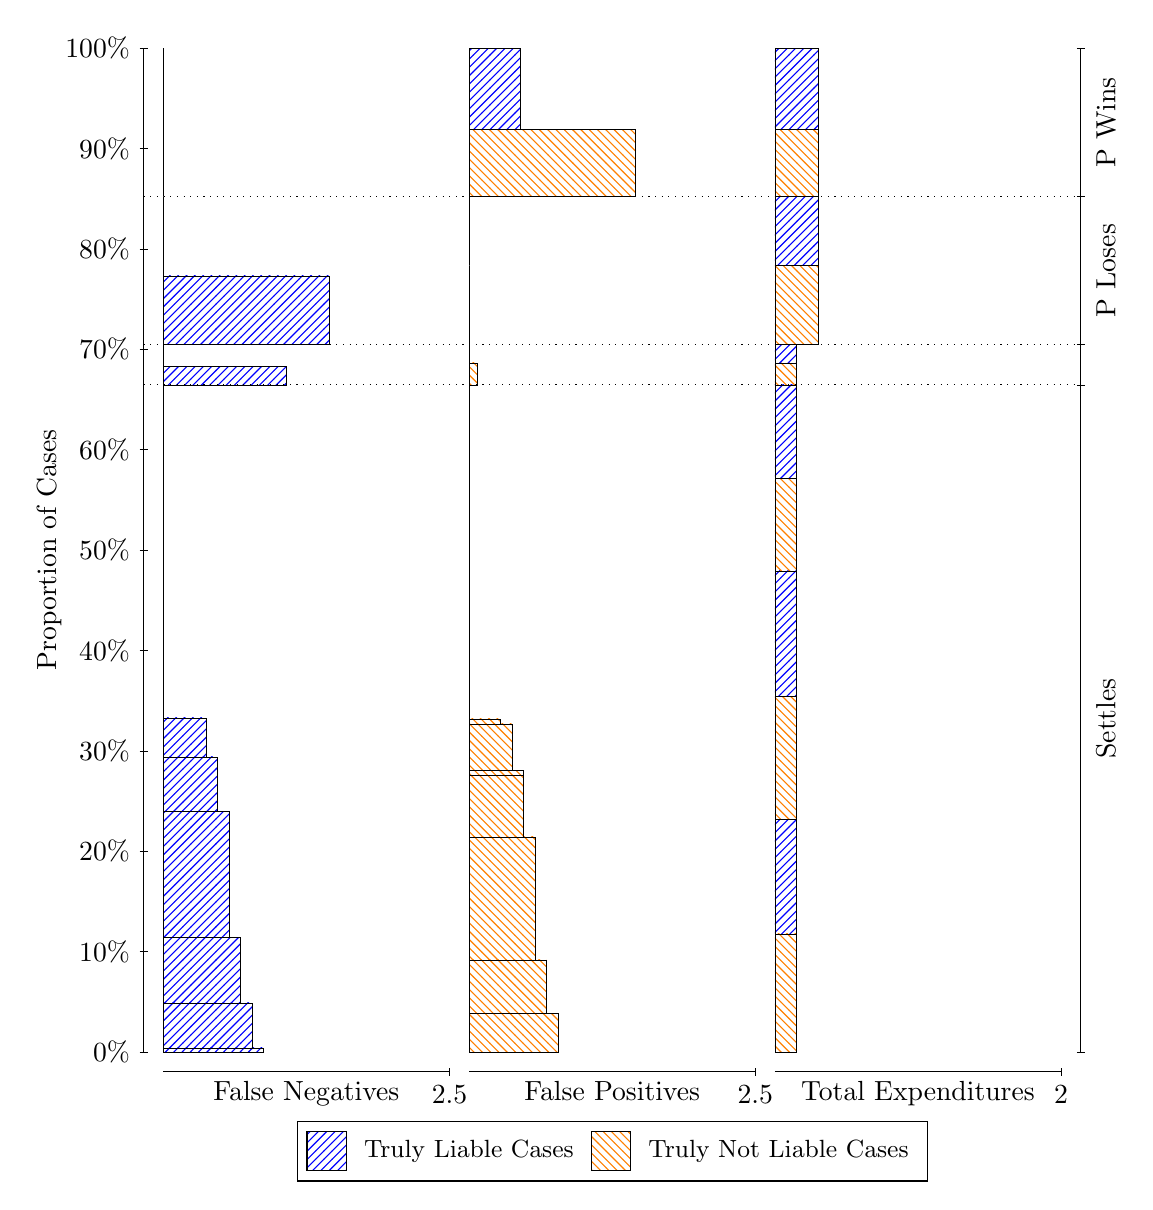
\begin{tikzpicture}
\draw[black, very thin] (1.5,1.75) -- (1.5,14.5);
\node[rotate=90, text=black, anchor=center] at (0.3, 8.125) {Proportion of Cases};
\draw[black, very thin] (1.45,1.75) -- (1.55,1.75);
\node[text=black, anchor=east] at (1.45, 1.75) {0\%};
\draw[black, very thin] (1.45,3.025) -- (1.55,3.025);
\node[text=black, anchor=east] at (1.45, 3.025) {10\%};
\draw[black, very thin] (1.45,4.3) -- (1.55,4.3);
\node[text=black, anchor=east] at (1.45, 4.3) {20\%};
\draw[black, very thin] (1.45,5.575) -- (1.55,5.575);
\node[text=black, anchor=east] at (1.45, 5.575) {30\%};
\draw[black, very thin] (1.45,6.85) -- (1.55,6.85);
\node[text=black, anchor=east] at (1.45, 6.85) {40\%};
\draw[black, very thin] (1.45,8.125) -- (1.55,8.125);
\node[text=black, anchor=east] at (1.45, 8.125) {50\%};
\draw[black, very thin] (1.45,9.4) -- (1.55,9.4);
\node[text=black, anchor=east] at (1.45, 9.4) {60\%};
\draw[black, very thin] (1.45,10.675) -- (1.55,10.675);
\node[text=black, anchor=east] at (1.45, 10.675) {70\%};
\draw[black, very thin] (1.45,11.95) -- (1.55,11.95);
\node[text=black, anchor=east] at (1.45, 11.95) {80\%};
\draw[black, very thin] (1.45,13.225) -- (1.55,13.225);
\node[text=black, anchor=east] at (1.45, 13.225) {90\%};
\draw[black, very thin] (1.45,14.5) -- (1.55,14.5);
\node[text=black, anchor=east] at (1.45, 14.5) {100\%};

\draw[black, very thin] (13.4,1.75) -- (13.4,14.5);
\draw[black, very thin] (13.35,1.75) -- (13.45,1.75);
\node[anchor=west] at (13.35, 1.75) {};
\draw[black, very thin] (13.35,10.223) -- (13.45,10.223);
\node[anchor=west] at (13.35, 10.223) {};
\draw[black, very thin] (13.35,10.732) -- (13.45,10.732);
\node[anchor=west] at (13.35, 10.732) {};
\draw[black, very thin] (13.35,12.613) -- (13.45,12.613);
\node[anchor=west] at (13.35, 12.613) {};
\draw[black, very thin] (13.35,14.5) -- (13.45,14.5);
\node[anchor=west] at (13.35, 14.5) {};

\draw[black, very thin, pattern color=blue, pattern=north east lines] (1.75,1.75) rectangle (3.0217,1.8018);
\draw[black, very thin, pattern color=blue, pattern=north east lines] (1.75,1.8018) rectangle (2.8763,2.3731);
\draw[black, very thin, pattern color=blue, pattern=north east lines] (1.75,2.3731) rectangle (2.731,3.2071);
\draw[black, very thin, pattern color=blue, pattern=north east lines] (1.75,3.2071) rectangle (2.5857,4.801);
\draw[black, very thin, pattern color=blue, pattern=north east lines] (1.75,4.801) rectangle (2.4403,5.4984);
\draw[black, very thin, pattern color=blue, pattern=north east lines] (1.75,5.4984) rectangle (2.295,5.9935);
\draw[black, very thin, pattern color=orange, pattern=north west lines] (1.75,5.9935) rectangle (1.75,10.223);
\draw[black, very thin, pattern color=blue, pattern=north east lines] (1.75,10.223) rectangle (3.3123,10.452);
\draw[black, very thin, pattern color=orange, pattern=north west lines] (1.75,10.452) rectangle (1.75,10.732);
\draw[black, very thin, pattern color=blue, pattern=north east lines] (1.75,10.732) rectangle (3.8573,11.605);
\draw[black, very thin, pattern color=orange, pattern=north west lines] (1.75,11.605) rectangle (1.75,12.613);
\draw[black, very thin, pattern color=orange, pattern=north west lines] (1.75,12.613) rectangle (1.75,13.471);
\draw[black, very thin, pattern color=blue, pattern=north east lines] (1.75,13.471) rectangle (1.75,14.5);
\draw[black, very thin, pattern color=orange, pattern=north west lines] (5.6333,1.75) rectangle (6.7597,2.2431);
\draw[black, very thin, pattern color=orange, pattern=north west lines] (5.6333,2.2431) rectangle (6.6143,2.9196);
\draw[black, very thin, pattern color=orange, pattern=north west lines] (5.6333,2.9196) rectangle (6.469,4.4808);
\draw[black, very thin, pattern color=orange, pattern=north west lines] (5.6333,4.4808) rectangle (6.3237,5.2625);
\draw[black, very thin, pattern color=orange, pattern=north west lines] (5.6333,5.2625) rectangle (6.3237,5.3268);
\draw[black, very thin, pattern color=orange, pattern=north west lines] (5.6333,5.3268) rectangle (6.1783,5.9164);
\draw[black, very thin, pattern color=orange, pattern=north west lines] (5.6333,5.9164) rectangle (6.033,5.9796);
\draw[black, very thin, pattern color=blue, pattern=north east lines] (5.6333,5.9796) rectangle (5.6333,10.223);
\draw[black, very thin, pattern color=orange, pattern=north west lines] (5.6333,10.223) rectangle (5.7423,10.502);
\draw[black, very thin, pattern color=blue, pattern=north east lines] (5.6333,10.502) rectangle (5.6333,10.732);
\draw[black, very thin, pattern color=orange, pattern=north west lines] (5.6333,10.732) rectangle (5.6333,11.74);
\draw[black, very thin, pattern color=blue, pattern=north east lines] (5.6333,11.74) rectangle (5.6333,12.613);
\draw[black, very thin, pattern color=orange, pattern=north west lines] (5.6333,12.613) rectangle (7.7407,13.471);
\draw[black, very thin, pattern color=blue, pattern=north east lines] (5.6333,13.471) rectangle (6.2873,14.5);
\draw[black, very thin, pattern color=orange, pattern=north west lines] (9.5167,1.75) rectangle (9.7892,3.2488);
\draw[black, very thin, pattern color=blue, pattern=north east lines] (9.5167,3.2488) rectangle (9.7892,4.7059);
\draw[black, very thin, pattern color=orange, pattern=north west lines] (9.5167,4.7059) rectangle (9.7892,6.2671);
\draw[black, very thin, pattern color=blue, pattern=north east lines] (9.5167,6.2671) rectangle (9.7892,7.861);
\draw[black, very thin, pattern color=orange, pattern=north west lines] (9.5167,7.861) rectangle (9.7892,9.0306);
\draw[black, very thin, pattern color=blue, pattern=north east lines] (9.5167,9.0306) rectangle (9.7892,10.223);
\draw[black, very thin, pattern color=orange, pattern=north west lines] (9.5167,10.223) rectangle (9.7892,10.502);
\draw[black, very thin, pattern color=blue, pattern=north east lines] (9.5167,10.502) rectangle (9.7892,10.732);
\draw[black, very thin, pattern color=orange, pattern=north west lines] (9.5167,10.732) rectangle (10.062,11.74);
\draw[black, very thin, pattern color=blue, pattern=north east lines] (9.5167,11.74) rectangle (10.062,12.613);
\draw[black, very thin, pattern color=orange, pattern=north west lines] (9.5167,12.613) rectangle (10.062,13.471);
\draw[black, very thin, pattern color=blue, pattern=north east lines] (9.5167,13.471) rectangle (10.062,14.5);
\draw[black, dotted] (1.5,10.223) -- (13.4,10.223);
\draw[black, dotted] (1.5,10.732) -- (13.4,10.732);
\draw[black, dotted] (1.5,12.613) -- (13.4,12.613);
\draw[black, very thin] (1.75,1.5) -- (5.3833,1.5);
\node[text=black, anchor=north] at (3.5667, 1.5) {False Negatives};
\draw[black, very thin] (5.3833,1.45) -- (5.3833,1.55);
\node[text=black, anchor=north] at (5.3833, 1.45) {2.5};

\draw[black, very thin] (5.6333,1.5) -- (9.2667,1.5);
\node[text=black, anchor=north] at (7.45, 1.5) {False Positives};
\draw[black, very thin] (9.2667,1.45) -- (9.2667,1.55);
\node[text=black, anchor=north] at (9.2667, 1.45) {2.5};

\draw[black, very thin] (9.5167,1.5) -- (13.15,1.5);
\node[text=black, anchor=north] at (11.333, 1.5) {Total Expenditures};
\draw[black, very thin] (13.15,1.45) -- (13.15,1.55);
\node[text=black, anchor=north] at (13.15, 1.45) {2};

\node[text=black, centered, rotate=90] at (13.72, 5.9865) {Settles};

\node[text=black, centered, rotate=90] at (13.72, 11.672) {P Loses};
\node[text=black, centered, rotate=90] at (13.72, 13.556) {P Wins};

\draw (7.449999999999999,1.5) node[draw=none] (baseCoordinate) {};
\begin{scope}[align=center]
        \matrix[scale=0.5, draw=black, below=0.5cm of baseCoordinate, nodes={draw}, column sep=0.1cm]{
            \node[rectangle, draw, minimum width=0.5cm, minimum height=0.5cm, pattern color=blue, pattern=north east lines] {}; &
            \node[draw=none, font=\small, text=black] (B) {Truly Liable Cases}; &
            \node[rectangle, draw, minimum width=0.5cm, minimum height=0.5cm, pattern color=orange, pattern=north west lines] {}; &
            \node[draw=none, font=\small, text=black] (B) {Truly Not Liable Cases}; \\
            };
\end{scope}

\end{tikzpicture}
\end{document}